\documentclass{mscs}
\usepackage[pdftex]{graphicx}
\usepackage{amsmath, amsfonts}
\usepackage{listings}
\usepackage{xcolor}
\newcommand{\Coq}{{\sc Coq}}
\newcommand{\ssr}{{\sc SSReflect}}
\newcommand{\C}[1]{\mbox{\lstinline`#1`}}
\newcommand\N[1]{\langle\mbox{\itshape\rmfamily\small #1}\rangle}
\newcommand{\iitem}{{\it i-item}}
\newcommand{\ditem}{{\it d-item}}
\let\L=\lstinline

\definecolor{dkblue}{rgb}{0,0.1,0.5} 
\definecolor{lightblue}{rgb}{0,0.5,0.5} 
\definecolor{dkgreen}{rgb}{0,0.4,0} 
\definecolor{dk2green}{rgb}{0.4,0,0} 
\definecolor{dkviolet}{rgb}{0.6,0,0.8}
\definecolor{shadethmcolor}{rgb}{0.9, 0.9,1}


\def\lstlanguagefiles{defManSSR.tex}
\lstset{language=SSR}

\lstset{moredelim=[is][\color{red}\bfseries\ttfamily\underbar]{|*}{*|}}
%Highlights metalevel expressions in italic rm font
\lstset{moredelim=*[is][\itshape\rmfamily]{/*}{*/}}



\begin{document}
\title{A formal study of Bernstein coefficients and polynomials}
\author[Y. Bertot, F. Guilhot and A. Mahboubi]{Yves Bertot,
  Fr\'ed\'erique Guilhot and Assia
  Mahboubi\thanks{This work has been partially funded by the FORMATH
    project, nr. 243847, of the FET program within the 7th Framework
    program of the European Commission.
}}

\maketitle

\section{introduction}
Bernstein coefficients provide a discrete approximation of polynomials
inside a bounded interval. As such they are useful tools to solve
problems like locating the roots of polynomials, isolating these roots
or solving systems of inequations with polynomial members.  In
computer aided design, they are also used intensively as they give an
efficient tool to draw curves that are controlled by points that users
can grab and drag, with instantaneous and intuitive feedback on the
shape the curve will take as the control points move around.
Bernstein coefficients are closely related to splines and Bezier curves
and they have a very simple geometrical interpretation, which we illustrate
in section \ref{sec:geometrybernstein}.

Bernstein coefficient are defined for a given polynomial, a given
degree, and a given interval. if the degree is \(n\), then
the coefficients form a sequence of size \(n+1\). In
this paper, we are interested in three important properties of these
coefficients:
\begin{enumerate}
\item if the coefficients taken in order exhibit exactly one sign change,
  then the polynomial is guaranteed to have exactly one root inside
  the interval.
\item  if all coefficients have the same sign, then the
  polynomial is guaranteed to have no root inside the interval
  for which they have been computed.
\item there is an easy method to compute Bernstein coefficients for
  the two intervals obtained when splitting a larger interval from the
  Bernstein coefficients for this larger interval.
\end{enumerate}

We describe a formal proof of these three properties,
concentrating on the second and third properties. These proofs will be
done in the setting of polynomials with the rational coefficients and
rational values.

in the following, we will assume that we are working with polynomials
whose roots are all simple. Starting from an arbitrary polynomial it
is easy to produce another polynomial with the same roots but all of
them simple, simply by dividing it by the greatest common divisor of
this polynomial and its derivative.


The main plan of the proof of the first property is to describe a
sequence of pairs \((I_0, P_0)\) to \((I_3, P_3)\), each pair
containing an interval and a polynomial, so that every root of
polynomial \(P_i\) inside \(I_i\) is in bijective correspondance with
a root of polynomial \(P_{i+1}\) in the interval \(I_{i+1}\).  The
first interval and the first polynomial are simply \(I\) and \(P\).
The last interval is \((0, +\infty)\) and the last polynomial is \(b_0
+ b_1 X + \cdots + b_n X^n\), where the coefficients \(b_i\) have the
same sign as the Bernstein coefficients.  Going from \(P_i\) to
\(P_{i+1}\) we apply a given transformation.  The first transformation
is a change of variable so that \(I_1\) is \((0,1)\) and \(P_1(x) =
P_0(x \times r + (1 - x) l)\).  The second transformation is so that
\(I_2\) is \((1,+\infty)\) and \(P_2(x) = 0\) exactly when \(P_1(1/x)
= 0\), as long as \(x\neq 0\).  The third transformation is a
translation so that \(I_3 = (0,+\infty)\) and \(P_3(x) = P_2(1+x)\).
We will show that the condition on Bernstein coefficients simply
boils down to Descartes' law of sign for polynomial \(P_3\) in the
case where there is exactly one sign change in this polynomial's coefficients.
This path from one polynomial to another is described in section~\ref{sec:Bernstein}.

Descartes' law of signs provides a sufficient criterion for the
existence of exactly one root for a polynomial
between 0 and \(+\infty\).  In its
most general form, this law
expresses a relation between the number of roots of a polynomial
between 0 and \(+\infty\) and the number of sign changes in the
coefficients of this polynomial.  The number of sign changes is larger
than the number of roots and the difference between the two numbers is
a multiple of 2.  Thus, if the number of sign changes is 1, there is
exactly one root between 0 and \(+\infty\).

For our development, we only prove the corollary  of
Descartes' law of signs for the case where there is only one sign
change.  Expressing Descartes' law on the coefficients of polynomial
\(P_3\) yields directly a law expressed in terms of sign changes for
Bernstein's coefficients of \(P\) with respect to the
interval\footnote{we name the bounds \(l\) for \emph{left} and \(r\) for
\emph{right}.}
\((l,r)\).   This proof is done in section~\ref{sec:descartes}.

Another part of our work is to describe dichotomy.  Knowing Bernstein
coefficients for a polynomial and a given interval, it is easy to
obtain the Bernstein coefficients for the two half intervals, using
an algorithm due to de Casteljau.  In the process, we increase
the precision of the approximation given by the Bernstein
coefficients.  De Casteljau's algorithm is a simple combinatorial
algorithm based on taking arithmetic means of successive coefficients.
To justify this combinatorial process we show in
section~\ref{sec:dicho} that Bernstein
coefficients actually are the coefficients of the polynomial in a
different basis from the usual monomials, called the {\em Bernstein basis}.

Most of our proofs were made using only rational numbers as numeric
values.  Thus, we work with a type of numbers where equality and
comparison are decidable and the process we describe can effectively
be used in a decision procedure.

When considering only rational numbers, the existence of roots takes a
different meaning: if a polynomial has a single simple real root in an
interval, this root may not be rational.  However, we can use a
corresponding property on rational numbers: there exists a
sub-interval inside which the absolute value of the slope is bounded
below, and such that the values of the polynomial at the sub-interval
bounds have opposite signs.  In a similar vein, the intermediate value
theorem does not hold with rational numbers, but a corresponding
statement, expressed as a bounded-value property, does.  Our proof
development relies on this approach.  We describe the formal aspects
of this approach to describing roots in section~\ref{sec:rational}.

Our work on Bernstein coefficients is an important stepping stone
to address various aspects of real algebraic numbers, decision
procedures for real arithmetic, and more ambitious algorithms like
cylindrical decomposition.

The formal work described in this paper has been performed using
the Coq system\cite{coqart}, with ssreflect extension
\cite{GONTHIER:2008:INRIA-00258384:4}.  We think some characteristics
of the proof system played a key role in making this development
possible.  We describe these key aspects in section~\ref{sec:formal}.

\section{Bernstein coefficients}
\label{sec:bernsteindef}
For an arbitrary natural number \(n\), we can consider the set of polynomials
of degree smaller than \(n\) as a vector space, and the monomials
\(x^k\), with \(0 \leq k \leq n\) constitue a basis, the standard basis,
of of this vector space.
If \(p\) is a polynomial with coefficients \(a_i\), then
\(p(x) = \sum_{i=0}^n a_i x^i\)  and the coefficients \(a_i\) are also the
coefficients of \(p\) in the standard basis.

For arbitrary numbers \(l\) and
\(r\), we can also consider the following polynomials, called
the {\em Bernstein polynomials for degree \(n\) and the interval
\((l,r)\)} for \(0 \leq k \leq n\)
\[P_b(n, l, r, k) = \binom{n}{k} \frac{(x-l)^{n-k}(r-x)^k}{r-l}^n.\]
These polynomials also constitue a basis of the vector space of polynomial
of degree \(n\), and we will usually call it the {\em Bernstein basis} leaving
the degree and the values \(l\) and \(r\) unspecified.
Every polynomial \(p\) also has a sequence of coefficients
\(b_i\), so that \(p(x) = \sum_{i=0}^n P_b(n,l,r,i)(x)\).  The coefficients
\(b_i\) are the Bernstein coefficients.

When \(l < r\), the Bernstein polynomials are positive and each polynomial
of index \(k\) reaches its maximum at the point \(d_k=l+\frac{(r-l)k}{n}\), so
that each coefficient \(b_k\) somehow has a dominant influence on the value
of the polynomial around \(d_k\).  Moreover, the coefficients
\(\binom{n}{k}\) included in the definition of \(P_b(n,k,r,k)\) are chosen
in such a way that the coefficient \(b_k\) would tend to have a value
close to the value of the polynomial in \(d_k\).  For instance, if the
\(p_1\) is the constant polynomial with value \(1\), then all its Bernstein
coefficients are equal to 1; similarly, if \(p_2\) is the identity polynomial,
and \(n\) is larger than \(0\),
then the Bernstein coefficients for \(p_2\)
are \(l + \frac{(r-l) k}{n}\), as can
be verified using the following computation:
\begin{eqnarray*}
\lefteqn{\sum_{i=0}^n \left(l + \frac{(r-l)i}{n}\right) \binom{n}{i} \frac{(x-l)^i (r-x)^{n-i}}
{(r-l)^n}}\\
&=& \sum_{i=0}^n l \binom{n}{i}\frac{(x-l)^i(r-x)^{n-i}}{(r-l)^n} +
\sum_{i=0}^n \frac{i}{n}\binom{n}{i}\frac{(x-l)^i(r-x)^{n-i}}{(r-l)^{n-1}}\\
&=& l \frac{((x -l) + (r - x))^n}{(r-l)^n} +\sum_{i=1}^n \binom{n-1}{i-1}\frac{(x-l)^i(r-x)^{n-i}}{(r-l)^{n-1}}\\
&=& l +{ (x-l)\sum_{i=0}^{n-1}\binom{n-1}{i} \frac{(x-l)^i(r-x)^{(n-1)-i}}
{(r-l)^{n-1}}}\\
&=& l + (x -l) \frac{((x-l) + (r - x))^{n-1}}{(r-l)^{n-1}} = x
\end{eqnarray*}
At the first equality sign, we distribute inside the first sum; in the
second term, we simplify the denominator with the numerator \((r-l)\).
At the second equality sign, we recognize that the first term contains
a binomial formula corresponding to \(((x-l)+(r-x))^n\); in the second
term, we recognize that the first element of the sum can be removed
because it is 0, also we recognize that \(\frac{i}{n}\binom{n}{i}\) is
\(\binom{n-1}{i-1}\) when \(i\neq 0\).  At the third equality sign,
we use the equality \((x-l)+(r-x)=r-l\) for the first term and
we factor out \((x-l)\) from the remaining indexed sum and re-index that sum.
We then recognize another binomial formula and can conclude.

\label{sec:geometrybernstein}
The Bernstein coefficients are related to a broken line (made of
contiguous straightline segments) which gives a rough approximation of the
polynomial's function graph.  More precisely, given the bounds \((l,r)\)
of the interval,
the bernstein coefficients \((b_0,\ldots, b_n)\) define a collection of points
with coordinates \(c_i = (l + i \frac{r-l}{n}, b_i)\) each of these points describes
the behavior of the polynomial when the input \(x\) is close to
\(l+i\frac{r-l}{n}\).  In a sense, Bernstein coefficients can be said to
{\em control} the behavior of the polynomial in some part of the interval.
This is why the points \(c_i\) are often called {\em control points}.
These points can
be move about the vertical line \(x=l + i\frac{r-l}{n}\).  When \(b_i\) is
close to the average between \(b_{i-1}\) and \(b_{i+1}\) (in other words, when
\(c_i\) is close to the segment joining \(c_{i-1}\) and \(c_{i+1}\)), the
behavior of the polynomial in this area is quite eventless.  But when \(c_i\)
is significantly removed from this segment, \(c_i\) appears to be pulling the
polynomial's curve in its direction, with the curve of the polynomial usually
crossing the vertical line \(x=l+i\frac{r-l}{n}\) between the segment and
the point \(c_i\).  This is illustrated in the Figure~\ref{control}.
\begin{figure}
\begin{center}
\begin{tabular}{ccc}
\includegraphics[width=.30\textwidth,clip=true, trim=2cm 4cm 1cm 6.3cm]
{control.pdf}&
\includegraphics[width=.30\textwidth,clip=true, trim=2cm 4cm 1cm 6.3cm]
{control2.pdf}&
\includegraphics[width=.30\textwidth,clip=true, trim=2cm 4cm 1cm 6.3cm]
{control3.pdf}\\
(a) 1, 3, -10, 1, 4, 1 & (b) 1, 3, -1, 1, 4, 1 & (c) 3, 0, 1, 10, -2, -1\
\end{tabular}
\end{center}
\caption{\label{control} Bernstein Control points and corresponding polynomial curves}
\end{figure}

In Figure~{(\ref{control}-a)} the illustration shows that a peak in
the disposition of the control points corresponds to a bend in the
polynomial's curve (the Bernstein coefficients are 1, 3, -10, 1, 4, 1
and -10 corresponds to a downward peak).  In this case, the peak
provokes two sign changes, which are reproduced in the shape of the
curve and correspond to the existence of two roots inside the
interval.  In Figure~(\ref{control}-b), the coefficients still exhibit
a downward peak with a negative coefficient, but the polynomial's
curve stays away from the x-axis and the two sign changes in the
Bernstein coefficients do not correspond to any real root for the
polynomial (this is a false alert).  In Figure~(\ref{control}-c),
there is on sign change, so that the first and last coefficients have
opposite signs.  In fact, the first and the last Bernstein
coefficients are equal to the values of the polynomial at the bounds
of the interval, so this imposes the existence of at least one root.
But because there is exactly one sign change in the coefficients, we
can be sure that any other bend in the curve stays away of the x-axis.

\section{Describing roots of a polynomial in the rational setting}
\label{sec:rational}
In mathematics, we are accustomed to use several fields that have different
properties regarding the existence of roots of polynomials.  The most general
case is the the case of algebraically closed fields, like the fields of complex
numbers.  In these fields, any polynomial of degree larger than 1 and
with the coefficients in the field is guaranteed to have a root in the field.
For instance, any polynomial with complex coefficients is guaranteed to have
a root that is a complex number.

Then, we can consider an intermediary kind of fields, known as real closed
fields, like the field of real numbers.  These fields are
ordered and contain enough elements
so that they enjoy the existence of the {\em intermediate value theorem}:
any polynomial that has a negative value in one point \(a\) and a positive value
in another point \(b\) is guaranteed to have a root at some point between
\(a\) and \(b\).  The field of real numbers satisfies this property.

Then, we can consider smaller fields, like the field of rational numbers.
Here we don't have the {\em intermediate value theorem} anymore.  Still, it
makes sense to say that a bounded interval in the field of rational number
may contain exactly one root because the polynomial's curve crosses the
x-axis in exactly one point, which can be approximated arbitrarily close,
even if it does not really exist in the field of rational numbers.  This
what we want to make precise in the next two sections.


\subsection{Criteria for the existence of a unique root}
We concentrate on a sufficient criterion for the existence of a root
inside an interval.  This criterion is strong enough to build a Cauchy
sequence whose limit in the real numbers would be the root.  Our
criterion is based on slopes.

Ensuring that the slope is positive or negative is some interval helps
making sure that there are not two roots.  In our setting, where the
polynomials we consider have only simple roots, we have a stronger
property that the slope is separated from 0 by a given ratio.  In the
case of positive slopes, we write the slope requirement for a
polynomial \(p\) inside a given interval \(I\) as follows:
\[\exists k, 0 < k \wedge \forall x y, x \in I \wedge y \in I
\wedge x < y \Rightarrow k(y - x) < p(y) - p (x) \]

Depending on the kind of interval that we will consider, we will have
two different ways to express the existence of a single root in the
interval.

\begin{enumerate}
\item If the interval is bounded, we express that the interval can be
  decomposed into three parts, the first part where the polynomial's
  value is always negative (\(I_1\) in Figure~\ref{bounded_decompose}, the second part where the polynomial's
  value goes from negative to positive with a requirement on the
  slope (\(I_2\) in Figure~\ref{bounded_decompose}, and the third part where the polynomial's value is always
  positive (\(I_3\) in Figure \ref{bounded_decompose}).
\begin{figure}\label{bounded_decompose}
\begin{center}
\includegraphics[clip=true,trim= 2cm 7cm 0cm 9cm,scale=0.3]{bounded_decompose.pdf}
\end{center}
\caption{A sufficient criterion for the existence of a single root in a bounded interval}
\end{figure}
\item If the interval is unbounded, we express that the interval can
  be decomposed into two parts, the first part where the polynomials
  value is always negative (\(I_1\) in
  Figure~\ref{unbounded_decompose}, and the second part where there is
  a requirement on the slope with a positive slope (\(I_2\) in
  Figure~\ref{unbounded_decompose}).
\begin{figure}\label{unbounded_decompose}
\begin{center}
\includegraphics[clip=true,trim=2cm 3cm 2cm 9cm, scale=0.3]{unbounded_decompose.pdf}
\end{center}
\caption{A sufficient criterion for the existence of a single root in an unbounded interval}
\end{figure}
\end{enumerate}
\subsection{Finding locations where a polynomial's value is
  arbitrarily small}
\label{ssec:civt}
While we can't be sure to produce a rational value on which the
polynomial of interest returns the zero value, we at least need to be
able to produce an input for which the polynomial's value is
arbitrarily small. In classical mathematics once we know that the
polynomial takes values of opposite sign at the bounds of an interval,
we know that there is a root for this polynomial in this interval,
thanks to the {\em intermediate value theorem}. For this work, we establish
a simplified constructive replacement of the intermediate value
theorem especially for polynomials.  The statement we prove has the following
form:
\[\forall p~x~y~\varepsilon, 0 < \varepsilon \rightarrow
p(x) < 0 \leq p(y) \rightarrow\\
\exists x'~ y', -\varepsilon \leq p(x') < 0 \leq p(y') \leq \varepsilon \wedge
x \leq x' < y' \leq y\]
We call this theorem the {\em constructive intermediate value theorem}.

We again rely on reasoning about slopes. First, we establish that the
slope of any polynomial is bounded in absolute value on any bounded
interval. This gives us a way to establish that polynomials
enjoy a property that is akin to but stronger
than uniform continuity. Starting from an interval \((l,r)\) and
a polynomial we can produce a coefficient \(k\) so that the variation
of the polynomial between two points \(x\) and \(y\) is smaller than
\(|k\times(y-x)|\).

For a given \(\varepsilon\), and assuming \(p(x) < 0 < p(y)\) we can
choose an \(n\) so that \(\frac{k(y-x)}{n} < \varepsilon\)
 We then consider the
\(n+1\) values \(a_i = x + \frac{i\times (y-x)}{n}\) and we solve a
discrete problem over the values \(a_i\).  We simply need to find the
largest prefix \(a_0, \ldots, a_{j-1}\) so that all values \(p(a_k\) in this
prefix are negative.  We can set \(x' =a_{j-1}\), because the next
value \(a_j\) is necessarily non-negative and
\(p(a_j) - p(x') < \varepsilon\), thus \(-\varepsilon < p(x') < 0\).
In a similar way, we can set \(y'= a_j\) because \(0 \leq p(y') < \varepsilon\).

Our algorithm is illustrated in figure~\ref{ivt}, where the distance
between the \(a_i\)'s is chosen according to the maximal slope
occurring between \(l=a_0\) and \(r=a_{12}\). The point selected by
our algorithm is \(a_6\), even though there are more roots in the
vicinity of \(a_1\) and \(a_2\) but neither \(a_1\) nor \(a_2\) is a
point where the polynomial takes a positive value.  The point \(a_{11}\) could
also be eligible, but it is not the smallest one.
\begin{figure}
\label{ivt}
\begin{center}
\includegraphics[clip=true,trim=0cm 9cm 2cm 9cm,scale=0.5]{ivt.pdf}
\end{center}
\caption{Bounding a polynomials value}
\end{figure}

\section{A simple form of Descartes' law of signs}\label{sec:descartes}
One of the main results studied in this paper
is that having only one sign changes in the
sequence of Bernstein coefficients for the polynomial \(p\) and the
interval \((l,r)\) ensures that there is only one root \(p\) inside
\((l,r)\).  The proof of this results relies on a similar property for
the standard coefficients of another polynomial \(p'\): if there is
only one sign change in the coefficients of \(p'\) then \(p'\) has
only one root inside the interval \((l,r)\).  In this section, we
discuss how this property is proved formally.

\subsection{A Geometrical explanation of the proof}
Let's first describe a simple graphical argument based on curves for polynomial functions between 0 and \(+\infty\), as shown in figure~\ref{graph-desc}.
\begin{figure}
\begin{center}
\includegraphics[width=0.5\textwidth]{alternated2.png}
\end{center}
{(a) non-negative coefficients, first one non-zero,\\
(b) non-negative coefficients, first one zero,\\
(c) first coefficient negative, all others non-negative,\\
(d) one sign change, first coefficient zero,\\
(e) one sign change, first coefficient negative}

\caption{\label{graph-desc}
Classes of polynomials with or without
sign change}
\end{figure}
To describe our proof, we assume that new polynomials are built from
existing ones by multiplying them by the polynomial \(X\) and adding a
constant; an operation that is known as ``Horner's scheme''.
Polynomials with one sign change and a positive principal coefficient
are obtained by starting with a positive constant, applying Horner's
scheme a certain number of times with non-negative constants, then
applying it a negative constant, and then applying it again a certain
number of times with non-positive constants.

Polynomials with only non-negative coefficients have curves which look
like the curves (\ref{graph-desc}-a) or (\ref{graph-desc}-b) depending on whether the first
coefficient is 0, adding a positive coefficient to a polynomial of the
form (\ref{graph-desc}-a) or (\ref{graph-desc}-b) yields a polynomial of the form (\ref{graph-desc}-a), multiplying a
polynomial of the form (\ref{graph-desc}-a) or (\ref{graph-desc}-b) by the polynomial \(X\) yields a new
polynomial of the form (\ref{graph-desc}-b).  Thus, Horner's scheme with non-negative
constants keeps polynomials in the (a-b) form.  Then, when applying
Horner's scheme with a negative coefficient (thus introducing a sign
change), the multiplication by \(X\) first builds a polynomial of the
(\ref{graph-desc}-b) form, and adding a negative constant, one obtains a curve whose
shape is given by (\ref{graph-desc}-c).  From then on, multiplying a polynomial of the
form (\ref{graph-desc}-c), (\ref{graph-desc}-d), or (\ref{graph-desc}-e) by \(X\) yields a a polynomial of the (\ref{graph-desc}-d) form; adding a
negative constant to a polynomial of the form (\ref{graph-desc}-d) or (\ref{graph-desc}-e) yields a
polynomial of the (\ref{graph-desc}-e) form.  Polynomials of the form (\ref{graph-desc}-d) or (\ref{graph-desc}-e)
share the following characteristic: there exists a positive value
\(x\), so that the polynomial has a negative value between 0 and
\(x\), and the slope of the curve is strictly positive above
\(x\).  Because of the slope condition, we can also find a point where
the polynomial is positive.

Let us now give a more precise proof, outlining the concepts that are
used in the formal proof.

\subsection{Lemmas for polynomials with non-negative coefficients}
Polynomials are simply encoded by their lists of coefficients, evaluating
a polynomials on a given number is done recursively following Horner's scheme,
and recognizing polynomials with only non-negative coefficients is also
done using a simple recursive function, written in the following form:
\begin{lstlisting}
  Fixpoint |*all_pos_or_zero*| (l:seq Qcb) : bool :=
  if l is a::tl then (0 <= a) && all_pos_or_zero tl else true.
\end{lstlisting}
As a reminder, the Coq syntax variant that we use, {\tt ssreflect},
privilegies boolean predicates, so that {\tt (0 <= a)} stands for a boolean
value computed by a recursive function instead of a proposition as in
standard Coq litterature.  Also, the type {\tt Qcb} stands for a
representation of
rational number as fractions in canonical form (hence the letter {\tt c}), where
the verification that the fraction is in canonical form is also expressed
using a boolean function (hence the letter {\tt c}).  Since these numbers
are in canonical form, the equality test between two fractions is simply based
on syntactic equality, in other words Leibnitz equality.  The type constructor
{\tt seq } is a type for lists, with extra constraints on the types
that can be
stored in such lists: equality must be decidable, a feature that can then be
exploited intensively by the {\tt ssreflect} package
\cite{GONTHIER:2008:INRIA-00258384:4}.

We should remark that polynomials satisfying the boolean predicate
{\tt all\_pos\_or\_zero} may not contain any positive coefficients: for this
reason, we cannot guarantee that they are increasing or strictly positive
anywhere between 0 and \(+\infty\).

We prove easily by induction on lists that if they contain only non-negative
coefficients, then the corresponding polynomial always has a postive value
in \((0,+\infty)\) and from then, we also prove by induction that
any polynomial with only non-negative coefficients is increasing.

We then prove that for every polynomial \(P\)  with non-negative coefficients,
the product \(x \times P(x)\) can be made arbitrarily close to 0.

\subsection{Two lemmas on slopes}
A first lemma on slopes concerns the existence of points where a
polynomial \(P\) takes a value above an arbitrary bound \(a\).  If the slope
is bounded below by a positive ratio \(k\), this is guaranteed as it
suffices to take a value that is large enough.  As the proof is
constructive, we need to be more precise: assuming the slope is larger
than \(k\) for any \(y\) larger than \(x_1\), it suffices to take any
value larger than \(x_1 + \frac{a - P(x_1)}{k}\).  This result is
remembered in our development under the name {\tt above\_slope}.

A second lemma on slopes concerns the slope of a product of the form
\(x \times P(x)\).  This
lemma reproduces the known formulas for the derivative of products of derivable
functions, but is expressed solely in terms of lower bounds of slopes.
{\sl if  a function \(f\) has a slope larger than or equal to a non-negative
ratio \(k_f\) when \(x\) is larger than a certain bound \(a\), then
then the slope of the product \(x \times f(x)\) is larger than
\(a k_f + f(x)\)}.

This statement requires \(f\) to have a positive slope, but it leaves open
whether \(f(x)\) is positive or not.  In particular, the values \(a\) and
\(k_r\) can be fixed for a large interval: we intend \(a\) to be the lower
bound of interval \(I_2\) as used in the criterion for existence of a unique
root in an unbounded interval (see Figure~\ref{unbounded_decompose}).

\subsection{Polynomials with exactly one sign change}
We can then address polynomials with exactly one sign change.  We want
to show that these polynomials have exactly one root.  We exhibit the
two intervals described in the criterion for unbounded intervals (see
Figure~\ref{unbounded_decompose}) the positive value \(x_1\) and the
positive ratio \(k\) such that the polynomial is negative in the
interval \((0, x_1)\) and the slope between any two values above
\(x_1\) is larger than \(k\).

To detect polynomial with exactly one sign changes, we use two recursive
functions.  The first one, which we call {\tt alternate\_1}, recognizes
polynomials with at least one positive coefficient, preceded by any number
of non-positive coefficients (possibly 0) and followed by only non-negative
coefficients, as checked by {\tt all\_pos\_or\_zero}.  This function is
defined as follows:
\begin{lstlisting}
Fixpoint alternate_1 (l:seq Qcb) : bool :=
  if l is a::tl then
     if 0 < a then all_pos_or_zero tl else alternate_1 tl
  else false.
\end{lstlisting}
The second function, which we call {\tt alternate}, checks for the
presence of at least one negative coefficient and then calls {\tt alternate\_1}.
Thus, {\tt alternate} calls itself recursively
as long as it finds zero coefficients, the function {\tt alternate\_1}
also calls itself recursively as long as it finds
non-positive arguments.

As we have two recursive functions, {\tt alternate\_1} and {\tt alternate},
we actually need to perform two proofs by induction.  Each proof by induction
shows that some invariant is satisfied.

The invariant for {\tt alternate\_1}
must be satisfied by a polynomial \(P\) that may or may not contain a negative
coefficient, so that this invariant cannot guarantee the existence of
places where the polynomial takes a negative value.  Instead, this invariant
guarantees for any positive \(\varepsilon\) the existence of a positive {\tt x}
and a \(k\) so that:
\begin{enumerate}
\item for any \(y\) between \(0\) and \(x\), \(P(y) \leq P (x)\) ,
\item the slope between two points larger \(x\) is guaranteed to be larger
than \(k\),
\item the number \(x \times P(x)\) is between \(0\) and \(\varepsilon\).
\end{enumerate}

The invariant for {\tt alternate} is exactly the criterion we use
to describe the existence of exactly one root in an unbounded interval.
This proof by induction is done by induction on the list.  The empty list
does not satisfy the predicate {\tt alternate} so that this case is
taken care of easily.  The other case is when the polynomial is described
by a list of the form {\tt \(a\)::\(l\)}, so that \(l\) represents another polynomial
\(P_l\) and \(P(x) = a + x \times P_l(x)\).  Here another case distinction mut be
studied, depending on whether \(a\) is zero or negative.

If \(a\) is negative, we cannot use an induction hypothesis, because in
this case \(l\) is only guaranteed to satisfy the predicate
{\tt alternate\_1}.  On the other hand, the invariant for {\tt alternate\_1}
guarantees the existence of an \(x\) so that \(x\times P_l(x)\) is positive
and smaller than \(-a\), this \(x\) is the right witness and the slope is
\(P_l(x)\).  Since \(P_l\) is negative at the left of \(x\) it is easy to
prove that \(y\times P_l(y)\) is negative when \(0 < y \leq x\), and thus
\(P(y)\) is negative.  To reason on the slope, we use our lemma about the
slope of \(x \times P(x)\), using \(0\) for the slope of \(P\) (we only
know that it is increasing).

If {\tt a} is
zero, we have by induction hypothesis that there exists an \(x\) and \(k\)
so that \(P_l\) is negative on the left of \(x\) and has a slope larger than
\(k\) on the right of \(x\).  However, this does not guarantee that \(x\) is
the right witness for \(P\) because the slope of \(x\times P_l(x)\) is only
larger than \(P_l(x) + x \times k\), and \(P_l(x)\) is negative.  The solution
is to note that \(P_l\) necessary takes a positive value in some point \(v1\)
on the right of \(x\) and to use our
{\em constructive intermediate value theorem} from
section~\ref{ssec:civt} to
build a new value \(x_1\) so that \(-\frac{k v_1}{2} \leq P_l(x_1) \leq 0\).
Now \(P_l\) is still guaranteed to be negative between \(x\) and \(x_1\),
because of the slope condition and now the slope on the right of \(x_1\) is
guaranteed to be larger than \(\frac{v1 k}{2}\), which is positive.

\section{From Bernstein to Descartes}\label{sec:Bernstein}
In this section, we clarify the polynomial transformations that link
the problem of finding the roots of a polynomial inside an arbitrary
bounded interval \((l,r)\) successively with the problem of finding
the roots of an other polynomial inside the interval \((0,1)\) and
with the problem of finding the roots of yet another polynomial inside
the interval \((0,+\infty)\).  These transformation make it possible to
compute another collection of coefficients, which happen to be very simply
related to Bernstein coefficients.

Proving the properties of Bernstein coefficients works by establishing
a route from Descartes' law of signs to Bernstein coefficients.  Descartes'
law of signs works for the interval \(0,+\infty\).  This criterion
can easily be adapted to any half-line interval \((a,+\infty)\) and
more precisely to \((1,+\infty)\).  Then a criterion on \((1,+\infty)\)
can be transformed into a criterion on \((0,1)\). This can, in turn,
be transposed to any interval.  It happens that this path gives a way to
reason on Bernstein coefficients.
\subsection{A criterion for the interval \((1,+\infty)\)}
The law of signs gives us a sufficient condition to determine when the
unbounded interval \((0,+\infty)\) contains exactly one root for a
polynomial. Through a change of variable, we obtain a similar
criterion for the interval \((1, +\infty)\).

In the following, we will call \(\theta_v\) the transformation that
maps any polynomial \(P\) to the polynomial \(y \mapsto P(y+v)\).  If
\(P=\sum_{i=0}^n a_i x^i\), We have the following formula:
\[P(y+a)= \sum_{i=0}^{n} a_i (y+v)^i = \sum_{k=0}^{n}
(\sum_{i=k}^{n}a_i\left(\begin{array}{c}i\\k\end{array}\right) v^{i-k}) y^k\]

The polynomial \(P\) has exactly one root in the interval \((v,+\infty)\)
if  and only if
the polynomial \(\theta_v(P)\) has exactly one root in the interval
\((0,+\infty)\).  This is particularly interesting for the case where
\(v=1\).  We proved this lemma, using our criterion for a unique root
in an unbounded interval to express the existence of root.

Thus, if we apply Descartes's law of signs on the coefficients
\(\sum_{i=k}^{n}a_i\left(\begin{array}{c}i\\k\end{array}\right)\), we
can obtain a sufficient criterion for the existence of exactly one
root of polynomial \(P=\sum_{i=0}^{n}a_ix^i\) in the interval
\((1,+\infty)\).
\subsection{A criterion for the interval \((0,1)\)}
Descartes' law of signs works for unbounded intervals.  In this
section, we see how to cover also bounded intervals. The trick here relies
on reversing the polynomial's list of coefficients.  Obviously, the
number of sign changes in a list of coefficients is the same as the
number of sign changes in the reversed list.

However, the roots of a polynomial on the interval \((1,+\infty)\)
are in one-to-one correspondence with the roots of the
reversed polynomial between zero and one. This is due to the following
equation:
\[\sum_{i=0}^{n}a_i x^i = x^n\times\sum_{i=0}^{n}a_i x^{i-n}\]
We can now perform another change of variable, here \(y=1/x\) and a
change of index \(j=n-i\) in the sum.
\[\sum_{i=0}^{n}a_i x^l = (\frac{1}{y})^n \sum_{j=0}^{n}a_{n-j} y^j\]
The polynomial \(\sum_{j=0}^{n} a_{n-j}y^j\) is exactly the reversed
polynomial, and the expression \((\frac{1}{y})^n\) never becomes 0 for
\(y\in (0,1)\).  Thus, \(x\) is a root of the polynomial between \(1\)
and \(+\infty\) if and only if \(y=x^-1\) is a root of the reversed
polynomial between \(0\) and \(1\).

Let us note \(\rho\) the function that computes the reverse of a
polynomial.  Here we need to be precise: the coefficients of a
polynomial of degree \(n\) actually are the coefficients of a vector
in an \(n+1\) dimensional space, whose basis is made of the monomials
\(X^i\) where \(i\in\{0,n\}\).  Seen as an operation on this vector
space, \(\rho\) is an automorphism and is its own inverse.  But
polynomials of degree less than \(n\) are also elements of this vector
space and the reverse operation must be understood as reversing the
list of coefficients of length \(n+1\) obtained by completing the
polynomials description with enough 0 coefficients.


To illustrate the correspondance between a polynomial and its reverse,
we can consider the polynomial \(P(x) = x^3 - 5/2 x^2 - 2 x + 3/2\),
the reversed polynomial is \(Q(x) = 3/2 x^3 - 2 x^2 - 5/2 x + 1\) and after
the variable change we obtain the polynomial \(3/2 x^3 + 5/2 x^2 - 2 x - 2\)
which exhibits only one sign change.  This predicts that the polynomial has
exactly one root between 0 and 1, and indeed the three roots of the initial
polynomial are -1, 1/2, and 3.  This is illustrated in
figure~\ref{invert} where the curve with a solid line is the curve for the
polynomial \(P\), while the curve with a dashed line is the curve for
the polynomial \(Q\), which has a single root between 1 and \(+\infty\).
\begin{figure}\label{invert}
\begin{center}
\includegraphics[clip=true,trim=3cm 5cm 3cm 14cm, width=0.5\textwidth]{invert.pdf}
\end{center}
\caption{Curves of \(x^3 -\frac{5}{2} x^2 - 2 x +
  \frac{3}{2}\) (solid line)
and its reverse \(\frac{3}{2}x^3 -2 x^2 - \frac{5}{2} x + 1\) (dashed)}
\end{figure}

As a conclusion, we cal also establish a correspondance between unique
roots in \((1,+\infty)\) unique roots in \((0,1)\), but not for the
same polynomials.  When working on rational numbers, this
correspondance works by linking the criterion for unbounded intervals
with criterion for bounded interval.  This proof involves the
computation of slope for a \(x^np(1/x)\) from the slope of \(p\),
which makes it trickier than the rest.  This is a place where
our constructive intermediate value theorem plays a role.

\subsection{handling arbitrary bounded intervals}

The next step is to relate the roots of any polynomial inside an
arbitrary interval \((l,r)\) with the roots of another
polynomial inside the interval \((0,1)\).  This is done with another
change of variable, this time \(x= (r-l) y + l\); in other words, the
polynomial function which maps any \(x\) to \(p(x)\) has a root
between \(l\) and \(r\) if and only if the polynomial function which
maps any \(y\) to \(p((r - l) y + l)\) has a root between 0 and 1.

Here again, we can define a generic transformation on polynomials,
named \(\chi_k\) that corresponds to expanding with a given ratio.
For an arbitrary polynomial \(P=\sum_{i=0}^n a_i X^i\), the polynomial
\(chi_k(p)\) is defined as follows:
\[chi_k(p) = \sum_{i=0}^n a_i(kX^i) = \sum_i{i=0}^n a_ik^i x^i\]

Thus, the change of variable to study the roots of polynomial \(p\)
is actually represented by \(\chi_{r-l}\circ \theta_l\).

The geometric effect of the polynomial transformation
is illustrated in figure~\ref{expand-translate}, where the shape
of the curve for the polynomial \(\frac{x^3}{8} - \frac{x^2}{8} + 3
x\) inside the interval \((2,4)\) is reproduced by the shape of the
curve for the polynomial \(x^3 -\frac{5}{2}x^2-2x+\frac{3}{2}\) inside
the theorem \((0,1)\).
\begin{figure}
\begin{center}\label{expand-translate}
\includegraphics[clip=true,trim=4.5cm 18cm 2cm 3cm, width=0.5\textwidth]{expand-translate.pdf}
\end{center}
\caption{Curves of a polynomial inside \((2,4)\) and the
  corresponding transformed polynomial between \((0,1)\)}
\end{figure}
\subsection{Recapitulating operations}\label{ssec:ops}
In our formal development, we defined the three operations for
translating (\(\theta\)), expanding (\(\chi\)),
 and reversing the list of coefficients (\(\rho\)).  We can then
compute a sequence of coefficients by applying the transformation
\[\theta_1\circ\rho\circ \chi_{r-l}\circ_{l}\]

The coefficients we obtain satisfy this equality, which can be compared
with the definition of Bernstein coefficients from
section~\ref{sec:bernsteindef}.
It appears that the coefficients \(c_i\) that one obtains through this
process are
The
Bernstein coefficients for a polynomial \(p\)  an interval \((l,r)\)
are then obtained by, first expanding (composing \(p\) with
\(x\mapsto (r-l) x + l\), then reversing the list of coefficients, and
then translating, i.e. composing with \(x \rightarrow x - 1\).  The
coefficients we obtain through this process, \(c_i\) are related to the
Bernstein coefficients \(b_i\)
in the sense that \(c_i = \left(\begin{array}{c}i\\n
\end{array}\right)b_i\), thus their sign is exactly the sign of the
Bernstein coefficients.  It is thus enough to reason on the signs of
the coefficients \(c_i\).  We show that one sign changes in these coefficients
is sufficient to ensure the existence of exactly one root in the interval
\((l,r)\).  In particular:

\begin{itemize}
\item translating a polynomial preserves the criterion for existence
of exactly one root in bounded intervals and in unbounded intervals,
\item expanding a polynomial preserves the criterion for existence of
  exactly one root in bounded intervals,
\item reversing the list of coefficients maps a polynomial satisfying
  the criterion for the existence of exactly one root in the unbounded
  interval \((1,+\infty)\) into a polynomial satisfying the criterion
  for the existence of exactly one root in the bounded interval \((0,1)\).
\end{itemize}

\section{Dichotomy}
\label{sec:dicho}
Bernstein coefficients give precise information when they exhibit
either zero or one sign change. in the first case, we have the
guarantee that there are no roots of the considered polynomial in the
considered interval. In the second case, we have the guarantee that
there is exactly one root.

When Bernstein coefficients exhibit more than one sign change, no
conclusion can be drawn about the existence and unicity of roots in the
interval.  For instance, in Figure~(\ref{control}.b), the Bernstein
coefficients exhibit two sign changes, but there is no root inside the
interval.  When facing this kind of unconclusive information, the solution
is to refine the approximation given by the control line.

\subsection{Geometric intuition for dichotomy}
\label{ssec:dichogeom}
When cutting an interval in two halves, the number of control points is
approximately doubled, because each of the new half-intervals receives a
new sequence of \(n\) bernstein coefficients.  As a result, the control points
are closer to each other and to the polynomial's curve and they give a more
accurate account of the curve's position with respect to the x-axis.  This is
illustrated in Figure~\ref{dichotomy-curve}, where the initial Bernstein
coefficients exhibit a sign change, which is needed to account for the bend
in the first half of the interval (a positive local minimal, but expressed
by a negative Bernstein coefficient).  In the halved interval two more points
are added in the vicinity of the bend, and none of the control points needs
to be negative anymore.
\begin{figure}
\begin{center}
\includegraphics[clip=true,trim=2cm 12cm 1cm 11cm,width=0.6\textwidth]{control4.pdf}
\caption{\label{dichotomy-curve}Bernstein control points for halved intervals}
\end{center}
\end{figure}

In Figure~\ref{dichotomy-curve}, the dotted line represents
the polynomial's curve, the solid line links the control points for
the largest interval, marked by round bullets (the Bernstein coefficients are
1, 3, -1, 1, 4 1 for this interval).  The dashed line links the control points
for the two half intervals, marked by square boxes
(the Bernstein coefficients are 1, 2, 1.5, 1,
0.9375, 1.15625 for the first interval, and 1.15625, 1.375, 1.875, 2.5, 2.5,
1 for the second interval).  This figure illustrates that the control line
really gets closer to the polynomial's curve, and provides a much better
approximation of the polynomial.

The formula given in section~\ref{sec:bernsteindef} is useful to compute an
initial series of Bernstein coefficients, and the correctness of the
conditions for existence of roots based on these coefficients can be
justified using the transformation described in
section~\ref{ssec:ops}.

It appears that computing Bernstein polynomials is a costly process.
Around 1950, De Casteljau noticed that the coefficients for the sub intervals
were easy to compute from the coefficients for the big interval
through a simple recursive process. We have also proved the
correctness of this algorithm. This proof is the topic of the next
section.

\subsection{Bernstein Bases}
\label{ssec:basis}
As soon as \(r\) and \(l\) are different, The transformations used in
section \ref{ssec:ops} are all inversible.
The inverse of translating by a constant \(a\) is translating by
the constant \(a\), the inverse of reversing a list of coefficients
is reversing again, and the inverse of expanding by a ratio \(k\) is
expanding by the ratio \(k^{-1}\).

\subsection{splitting algorithm}\label{ssec:split}

Given three pairwise distinct rational numbers $a, b, m$,
there exists an efficient algorithm to deduce the two respective lists
of Bernstein coefficients of a polynomial $P$ on intervals $(a, m)$
and $(m, b)$ from the list of Bernstein coefficients of $P$ on
interval $(a, b)$.

Let \C{c} be the sequence of Bernstein coefficients of a polynomial $q$
for an interval \((a,b)\) with \(a, b\in \mathbb{Q}\) and degree \(n\).
Let $m\in \mathbb{Q}$ be a rational number
distinct from $a$ and $b$. We pose
$\alpha := \frac{m - a}{b - a}$ and $\beta := \frac{b - m}{b -a}$. The
\C{|*de_casteljau*|} algorithm is defined recursively by:
\begin{lstlisting}
  Fixpoint |*de_casteljau*| (alpha beta : Qcb) (c : nat -> Qcb) (n : nat) :=
    match n with
    | O => b
    | i.+1 => fun j =>
      (alpha * de_casteljau c i j + beta * de_casteljau c i j.+1)
  end.
\end{lstlisting}
where the initial sequence of coefficients \C{c} is represented by an
infinite sequence of rational numbers, for which only the $p$ first
elements are relevant.
It computes the two expected new Bernstein coefficients lists:
\begin{lstlisting}
  Definition |*dicho'*| alpha beta c i :=
    de_casteljau alpha beta c i 0.
\end{lstlisting}
give the Berstein coefficients of $P$ on the finite interval with
bounds $a$ and $m$, and:
\begin{lstlisting}
  Definition |*dicho*| alpha beta p c i :=
     de_casteljau alpha beta c (p - i) i.
\end{lstlisting}
gives the Bernstein coefficients of $P$ on the finite interval with
bounds $m$ and $b$. Note that if in our case, we will only use the de
Casteljau algorithm with $m$ the midpoint of the initial interval, we
do not make here any assumption on the respective positions of $a, b$
and $m$. The aim of this section is to prove that this algorithms is
correct, i.e. that the \C{|*dicho*|} and \C{|*dicho'*|} function
indeed computes the expected Bernstein coefficients. The correctness
theorems as stated in \Coq{} are:
\begin{lstlisting}
Lemma |*dicho'_correct*| : forall (a b m : Qcb)(q : {poly Qcb})(p : nat)
(c : nat -> Qcb)
(alpha := (b - m) * (b - a)^-1) (beta := (m - a) * (b - a)^-1),
  m != a ->
  q = \sum_(i < p.+1)(c i) * bernp a b p i ->
  q = \sum_(j < p.+1)(dicho' alpha beta c j) * bernp a m p j.

Lemma |*dicho_correct*| : forall (a b m : Qcb)(q : {poly Qcb})(p : nat)
(c : nat -> Qcb)
(alpha := (b - m) * (b - a)^-1) (beta := ((m - a) * (b - a)^-1)),
  m != b ->
  q = \sum_(i < p.+1)(c i) * bernp a b p i ->
  q = \sum_(j < p.+1)(dicho alpha beta p c j) * bernp m b p j.
\end{lstlisting}
where \C{(bernp a b p i)} is the $i$-th polynomial in the Bernstein
basis of degree $p$ with paramters $a$ and $b$.
\begin{figure}[ht]\label{bern}
\begin{center}
\includegraphics[width=0.5\textwidth]{bern1.pdf}
\end{center}
\caption{Properties of de Casteljau computations}
\end{figure}


The properties of computations performed by the de Casteljau algorithm
are summarized on Figure \ref{bern}. Starting from the input list
$c := (b_0^(0)\dots b_p^{(0)})$ of coefficients in the basis with
parameters $a$ and $b$, on the upper side of the triangle, it
computes the full triangle, so that in the end the two expected output
lists can be read on the two  other sides of the triangle. The list
$c' := b_0^{(0)} \dots b_0^{(j)} \dots b_0^{(p)}$ is the list of
coefficients in the basis with parameters $a$ and $m$ output by
\C{dicho'}. The list
$c'' := b_0^{(p)} \dots b_j^{(p - j)} \dots b_p^{0}$
 is the list of coefficients in the basis with parameters $m$ and $b$
 output by \C{dicho}.  The green area on Figure \ref{bern} show which values
a the computation of an arbitrary given point in the triangle relies on.
This structure is imposed by the fixpoint
 equation of the recursive definition of the de Casteljau algorithm:
\begin{lstlisting}
  de_casteljau alpha beta c n.+1 i =
  (de_casteljau alpha beta c n i) + (de_casteljau alpha beta c n i.+1)
\end{lstlisting}
which looks very similar to the recursive relation governing the
Pascal triangle.

Let us first notice that the shape of Bernstein polynomials implies
that:
\begin{lstlisting}
Lemma |*bern_swap*| :
 forall p i l r,
 (i <= p) -> r != l ->  bernp r l p i = bernp l r p (p - i).
\end{lstlisting}
This remark implies that if $c$ is the list of coefficients of the
polynomial $q$ in the Bernstein basis of degree $p$ with parameters
$a$ and $b$, then the reverse of $c$ is the list of coefficients of
the same polynomial $q$ in the Bernstein basis of degree $p$ with
parameters $b$ and $a$: reversing the list swaps the parameters:

\begin{lstlisting}
Lemma |*bern_rev_coef*| : forall (p : nat)(a b : Qcb)(c : nat -> Qcb),
  \sum_(i < p.+1)(c i) * (bernp a b p i) =
  \sum_(i < p.+1)(c (p - i)) * (bernp b a p i).
\end{lstlisting}
This remark shows that the correctness of the \C{dicho'} function is
enough to get a certified computation of both Bernstein coefficient
lists: if $c$ is the
initial list of Bernstein coefficients with parameters $a$ and $b$, then
reversing $c$ gives the  coefficients with parameters $b$ and $a$,
applying \C{dicho'} on the reverse of $c$ using $b$, $a$ amd $m$
computes the coefficients with parameter $b$ and $m$, hence reversing
this output gives the result expected for \C{dicho} on $c$ using $a$,
$b$ and $m$. Using a similar symmetry reasoning on the
\C{de_casteljau} algorithm, we in fact reduce the proof of the
\C{dicho_correct} specification to the proof of \C{dicho'_correct}.

By linearity, we can also reduce the proof of the \C{dicho'_correct}
specification to the case where the input polynomial $q$ is in fact
itself a Bernstein polynomial. This means that the input coefficient
list $c$ only contains zeros except at one position where the
coefficient is one.

Let us first compute the expected output of the \C{dicho'} function on
a such a list. In other words, for any distinct rational numbers $a,
b, m$ and any $p\in \mathbb{N}$, given $i \leq p$, we want to compute
the coefficients of:
$$Bern_{p, i}(a, b) := \binom{p}{i} \frac{(X - a)^i(X - b)^{p -i}}
{(b  - a)^p}$$ in the basis $(Bern_{p, i}(a, m))_{i = 0, \dots, p}$.
We pose
$\alpha := \frac{b -  m}{b - a}$ and $\beta := \frac{m - a}{b - a}$.
In the polynomials of the new basis, formal denominators are of the
form $(m - a)$. By noticing that:
$$\frac{X - a}{b - a} = \beta \frac{X - a}{m - a} \quad \textrm{and} \quad
\frac{b - X}{b - a} = \alpha\frac{X - a}{m - a} +\frac{m - X}{m - a}$$
and by using the binomial identity:
$$\binom{p}{i}\binom{p - i}{j - i}  = \binom{j}{i}\binom{p}{j}$$
we obtain that:
$$Bern_{p, i}(a, b) =
\sum_{j = i}^p\binom{j}{i}\alpha^{j-i}\beta^i Bern_{p, j}(a, m) \quad (*)$$
Now to achieve the proof of the \C{dicho'_correct} lemma, it is
sufficient to prove that the values output by the \C{dicho'} function
coincide with the ones of $(*)$, which boils down to an induction on $i$.

\section{Formalization issues}
\label{sec:formal}


\subsection{Algebraic structures}

This work is based on the hierarchy of algebraic structures available
in the \ssr{} repository. This hierarchy, described in \cite{hieralg},
has be since enriched with interfaces for ordered integral
domains. The ordered integral domains instances we use here are
integers and rational numbers. For this purpose, we have populated the
hierarchy with the adequate structures on the types provided by the
standard library of the \Coq{} system. The \ssr{} algebraic
structures require their carrier type to be equipped with a boolean
equality test reflecting the structural Leibniz equality available by
default on the type. In our case, since the only concrete types
(integers and rational numbers) we manipulate constructively fall into
this category, this was not a compromise. We have hence equipped
these standard \Coq{} datatypes with all the desirable \ssr{}
algebraic structures.

The libraries already present in the standard distribution of the
system were containing a sufficient body of lemmas to achieve this
formalization. But the \ssr{} layer of interfaces introduces a very
uniform framework to deal with algebraic manipulations. Instances of a
same interface in particular share theory, hence lemma names, and
notations. In what we have described so far, there are for instance
several ring structures involved, namely the ring of integers, the one
of rational numbers, and the ring of polynomial with rational
coefficients. Being all instances of the ring abstract interface, all
these structures share the same symbols for operations, like \C{(x * y)} for
multiplication of \C{x} by \C{y}, \C{(x *+ n)} for the product of \C{x}
by a natural number (which is in fact defined as iterated
additions). The latter operation is of special interest to deal with
binomial coefficients in a transparent way since the theory of
binomial coefficients, defined as natural numbers, directly applied
without any further injection.



\subsection{Representations of polynomials}

The point of this work is to study polynomials seen as functions
$\mathbb{Q} \rightarrow \mathbb{Q}$. But the criteria we use to study
the roots of polynomials are dealing with lists of coefficients, in
various bases. Sometimes it is desirable to envisage this list of
coefficients to be a finite list, and sometimes it is more convenient
to consider a coefficient function, regardless of the degree of the
polynomial it defines. In the case we consider polynomials as finite
lists of coefficients, it might be useful to normalize this list to
get a non zero leading coefficient as last element of the list
representing a non zero polynomial (we work with a big endian
representation): this allows to get a boolean comparison test for free
from the one available on coefficients. But in the case polynomials are
seen as linear combination of a monomial basis for polynomials of
degree less than a fixed values, zeros in the coefficients become
meaningful. And this occurs for instance in the de Casteljau algorithm.

The formal development has to take all these multiple low level
convenient representations into account not to introduce too much
noise in the proofs.

The algorithms of real root testing operate on bare lists of rational
numbers, seen as big endian lists of coefficients. But for the
specification of these operations, and specially
for the correctness of Bernstein coefficient computations with respect
to monomials, and by de Casteljau, we stand on the \ssr{} big endian
representation of polynomials as \emph{normalized} lists of
coefficients.

(here comes the Coq definition)

The big endian choice is well suited for Horner evaluation. The
monomial $X$ is hence represented by:


A polynomial can always be seen as a list of coefficients, because
there is a coercion from polynomial to lists. But an arbitrary list
can also be transformed into a polynomial by the \C{Poly} operator,
which removes the tail zeroes from the list, and pack it with a
well-formednedd proof. To use this \C{Poly} operator it is convenient
to dispose of lemmas on the behaviour of list iterators under the
\C{Poly} construction (ie. to specify their effect on the polynomial
built).

(here comes the Coq definition)

Polynomials are equipped with a ring structure as soon as their
coeffocoent type is. As an indirect consequence, the \ssr{} polynomial
library also allows to define a polynomials on a ring structure \C{R}
by providing its coefficient function \C{nat -> R}. This facility is
in fact a simple use of the iterated operator facilities available in
\ssr{} \cite{bigops}: such a polynomial is simply

(here comes the Coq definition)

where \L+\sum+ is a notation for the iteration of the addition of a
ring structure. In particular, such sums behave as expected
(associativity, commutativity) and combine well with the
\L+\prod+ iteration of the associated ring product.

A last issue to be adressed is the way polynomials are seen as linear
coefficients of a monomial or Bernstein basis of polynomials of degree
less than a fixed value. This requires potentially padding
the list of the above \C{poly} representation with some zeros. This
amount to formalizing the fact that polynomials of degree less than a
fixed value form a finite dimentional vector space and to specify the
changes in the basis. Unfortunately, the linear algebra part of the
\ssr{} archive is not yet sufficiently well integrated to get this
easily from an existing infrastructure. We hence only define these
linear algebra operation at a low level (catenating zeros,...) and
prove them correct, which certainly leaves room for improvement.


\subsection{Automatization issues}

The automation given by the type inference based infrastructure is
relieving the user from many painful formalization issues. Beside the
sharing of notation and theory mentioned above, which is automatically
infered on the fly, algebraic manipulation on indexed sums is a
routine work.

For instance, spliting sums or distributing the product by a constant,
even a natural number, is straightforward.

(examples comes here).

On the other side, a significant part of scripts is devoted to much
too atomic rewrite steps to normalize ring expressions, or prove trivial
consequences of the transitivity of order.

The issue on rings should be solvable: in fact \ssr{} ring structures
are not yet interfaced with \Coq{} automation tools like the \C{ring}
tactic. This tactic might furthermore be enhanced to be able to deal
simultaneously with the various ring structures that can be mixed in a
goal, like the ring of polynomials and the one of its coefficients.

(example comes here)

The issue on order statements shall be partially adressed by also
adapting \Coq{} automated tactics to \ssr{} structures. But in this
case, order is often combined with non linear expressions, for which
it is quite difficult to get a truely efficient proof producing decision
procedure. This is in fact the ultimate goal of the work. So may be
incomplete but lightweight tools should be crafted to relieve the user
when possible.

(cite the rational tactic?)

\section{Conclusion}
{\sf travaux reli�s: Bridges et Bishop sur la continuit� uniforme, qui est
�galement utilis�e dans nos travaux.}
\bibliographystyle{alpha}
\bibliography{biblio}


\end{document}
%%% Local Variables:
%%% mode: latex
%%% TeX-master: t
%%% End:
